\documentclass[1p]{elsarticle_modified}
%\bibliographystyle{elsarticle-num}

%\usepackage[colorlinks]{hyperref}
%\usepackage{abbrmath_seonhwa} %\Abb, \Ascr, \Acal ,\Abf, \Afrak
\usepackage{amsfonts}
\usepackage{amssymb}
\usepackage{amsmath}
\usepackage{amsthm}
\usepackage{scalefnt}
\usepackage{amsbsy}
\usepackage{kotex}
\usepackage{caption}
\usepackage{subfig}
\usepackage{color}
\usepackage{graphicx}
\usepackage{xcolor} %% white, black, red, green, blue, cyan, magenta, yellow
\usepackage{float}
\usepackage{setspace}
\usepackage{hyperref}

\usepackage{tikz}
\usetikzlibrary{arrows}

\usepackage{multirow}
\usepackage{array} % fixed length table
\usepackage{hhline}

%%%%%%%%%%%%%%%%%%%%%
\makeatletter
\renewcommand*\env@matrix[1][\arraystretch]{%
	\edef\arraystretch{#1}%
	\hskip -\arraycolsep
	\let\@ifnextchar\new@ifnextchar
	\array{*\c@MaxMatrixCols c}}
\makeatother %https://tex.stackexchange.com/questions/14071/how-can-i-increase-the-line-spacing-in-a-matrix
%%%%%%%%%%%%%%%

\usepackage[normalem]{ulem}

\newcommand{\msout}[1]{\ifmmode\text{\sout{\ensuremath{#1}}}\else\sout{#1}\fi}
%SOURCE: \msout is \stkout macro in https://tex.stackexchange.com/questions/20609/strikeout-in-math-mode

\newcommand{\cancel}[1]{
	\ifmmode
	{\color{red}\msout{#1}}
	\else
	{\color{red}\sout{#1}}
	\fi
}

\newcommand{\add}[1]{
	{\color{blue}\uwave{#1}}
}

\newcommand{\replace}[2]{
	\ifmmode
	{\color{red}\msout{#1}}{\color{blue}\uwave{#2}}
	\else
	{\color{red}\sout{#1}}{\color{blue}\uwave{#2}}
	\fi
}

\newcommand{\Sol}{\mathcal{S}} %segment
\newcommand{\D}{D} %diagram
\newcommand{\A}{\mathcal{A}} %arc


%%%%%%%%%%%%%%%%%%%%%%%%%%%%%5 test

\def\sl{\operatorname{\textup{SL}}(2,\Cbb)}
\def\psl{\operatorname{\textup{PSL}}(2,\Cbb)}
\def\quan{\mkern 1mu \triangleright \mkern 1mu}

\theoremstyle{definition}
\newtheorem{thm}{Theorem}[section]
\newtheorem{prop}[thm]{Proposition}
\newtheorem{lem}[thm]{Lemma}
\newtheorem{ques}[thm]{Question}
\newtheorem{cor}[thm]{Corollary}
\newtheorem{defn}[thm]{Definition}
\newtheorem{exam}[thm]{Example}
\newtheorem{rmk}[thm]{Remark}
\newtheorem{alg}[thm]{Algorithm}

\newcommand{\I}{\sqrt{-1}}
\begin{document}

%\begin{frontmatter}
%
%\title{Boundary parabolic representations of knots up to 8 crossings}
%
%%% Group authors per affiliation:
%\author{Yunhi Cho} 
%\address{Department of Mathematics, University of Seoul, Seoul, Korea}
%\ead{yhcho@uos.ac.kr}
%
%
%\author{Seonhwa Kim} %\fnref{s_kim}}
%\address{Center for Geometry and Physics, Institute for Basic Science, Pohang, 37673, Korea}
%\ead{ryeona17@ibs.re.kr}
%
%\author{Hyuk Kim}
%\address{Department of Mathematical Sciences, Seoul National University, Seoul 08826, Korea}
%\ead{hyukkim@snu.ac.kr}
%
%\author{Seokbeom Yoon}
%\address{Department of Mathematical Sciences, Seoul National University, Seoul, 08826,  Korea}
%\ead{sbyoon15@snu.ac.kr}
%
%\begin{abstract}
%We find all boundary parabolic representation of knots up to 8 crossings.
%
%\end{abstract}
%\begin{keyword}
%    \MSC[2010] 57M25 
%\end{keyword}
%
%\end{frontmatter}

%\linenumbers
%\tableofcontents
%
\newcommand\colored[1]{\textcolor{white}{\rule[-0.35ex]{0.8em}{1.4ex}}\kern-0.8em\color{red} #1}%
%\newcommand\colored[1]{\textcolor{white}{ #1}\kern-2.17ex	\textcolor{white}{ #1}\kern-1.81ex	\textcolor{white}{ #1}\kern-2.15ex\color{red}#1	}

{\Large $\underline{12a_{0111}~(K12a_{0111})}$}

\setlength{\tabcolsep}{10pt}
\renewcommand{\arraystretch}{1.6}
\vspace{1cm}\begin{tabular}{m{100pt}>{\centering\arraybackslash}m{274pt}}
\multirow{5}{120pt}{
	\centering
	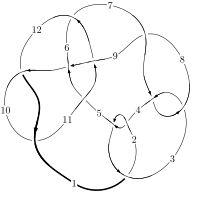
\includegraphics[width=112pt]{../../../GIT/diagram.site/Diagrams/png/912_12a_0111.png}\\
\ \ \ A knot diagram\footnotemark}&
\allowdisplaybreaks
\textbf{Linearized knot diagam} \\
\cline{2-2}
 &
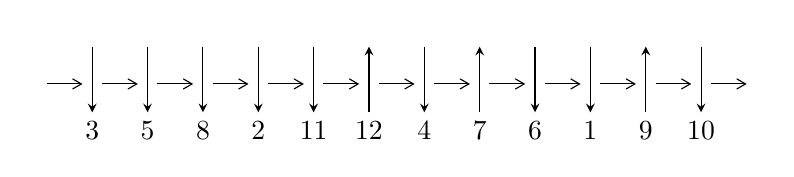
\begin{tikzpicture}[x=20pt, y=17pt]
	% nodes
	\node (C0) at (0, 0) {};
	\node (C1) at (1, 0) {};
	\node (C1U) at (1, +1) {};
	\node (C1D) at (1, -1) {3};

	\node (C2) at (2, 0) {};
	\node (C2U) at (2, +1) {};
	\node (C2D) at (2, -1) {5};

	\node (C3) at (3, 0) {};
	\node (C3U) at (3, +1) {};
	\node (C3D) at (3, -1) {8};

	\node (C4) at (4, 0) {};
	\node (C4U) at (4, +1) {};
	\node (C4D) at (4, -1) {2};

	\node (C5) at (5, 0) {};
	\node (C5U) at (5, +1) {};
	\node (C5D) at (5, -1) {11};

	\node (C6) at (6, 0) {};
	\node (C6U) at (6, +1) {};
	\node (C6D) at (6, -1) {12};

	\node (C7) at (7, 0) {};
	\node (C7U) at (7, +1) {};
	\node (C7D) at (7, -1) {4};

	\node (C8) at (8, 0) {};
	\node (C8U) at (8, +1) {};
	\node (C8D) at (8, -1) {7};

	\node (C9) at (9, 0) {};
	\node (C9U) at (9, +1) {};
	\node (C9D) at (9, -1) {6};

	\node (C10) at (10, 0) {};
	\node (C10U) at (10, +1) {};
	\node (C10D) at (10, -1) {1};

	\node (C11) at (11, 0) {};
	\node (C11U) at (11, +1) {};
	\node (C11D) at (11, -1) {9};

	\node (C12) at (12, 0) {};
	\node (C12U) at (12, +1) {};
	\node (C12D) at (12, -1) {10};
	\node (C13) at (13, 0) {};

	% arrows
	\draw[->,>={angle 60}]
	(C0) edge (C1) (C1) edge (C2) (C2) edge (C3) (C3) edge (C4) (C4) edge (C5) (C5) edge (C6) (C6) edge (C7) (C7) edge (C8) (C8) edge (C9) (C9) edge (C10) (C10) edge (C11) (C11) edge (C12) (C12) edge (C13) ;	\draw[->,>=stealth]
	(C1U) edge (C1D) (C2U) edge (C2D) (C3U) edge (C3D) (C4U) edge (C4D) (C5U) edge (C5D) (C6D) edge (C6U) (C7U) edge (C7D) (C8D) edge (C8U) (C9U) edge (C9D) (C10U) edge (C10D) (C11D) edge (C11U) (C12U) edge (C12D) ;
	\end{tikzpicture} \\
\hhline{~~} \\& 
\textbf{Solving Sequence} \\ \cline{2-2} 
 &
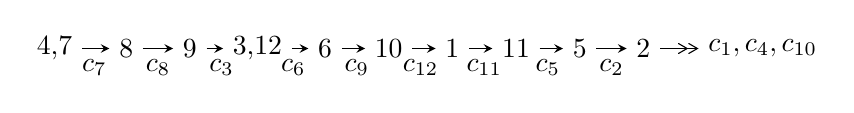
\begin{tikzpicture}[x=23pt, y=7pt]
	% node
	\node (A0) at (-1/8, 0) {4,7};
	\node (A1) at (1, 0) {8};
	\node (A2) at (2, 0) {9};
	\node (A3) at (49/16, 0) {3,12};
	\node (A4) at (33/8, 0) {6};
	\node (A5) at (41/8, 0) {10};
	\node (A6) at (49/8, 0) {1};
	\node (A7) at (57/8, 0) {11};
	\node (A8) at (65/8, 0) {5};
	\node (A9) at (73/8, 0) {2};
	\node (C1) at (1/2, -1) {$c_{7}$};
	\node (C2) at (3/2, -1) {$c_{8}$};
	\node (C3) at (5/2, -1) {$c_{3}$};
	\node (C4) at (29/8, -1) {$c_{6}$};
	\node (C5) at (37/8, -1) {$c_{9}$};
	\node (C6) at (45/8, -1) {$c_{12}$};
	\node (C7) at (53/8, -1) {$c_{11}$};
	\node (C8) at (61/8, -1) {$c_{5}$};
	\node (C9) at (69/8, -1) {$c_{2}$};
	\node (A10) at (11, 0) {$c_{1},c_{4},c_{10}$};

	% edge
	\draw[->,>=stealth]	
	(A0) edge (A1) (A1) edge (A2) (A2) edge (A3) (A3) edge (A4) (A4) edge (A5) (A5) edge (A6) (A6) edge (A7) (A7) edge (A8) (A8) edge (A9) ;
	\draw[->>,>={angle 60}]	
	(A9) edge (A10);
\end{tikzpicture} \\ 

\end{tabular} \\

\footnotetext{
The image of knot diagram is generated by the software ``\textbf{Draw programme}" developed by Andrew Bartholomew(\url{http://www.layer8.co.uk/maths/draw/index.htm\#Running-draw}), where we modified some parts for our purpose(\url{https://github.com/CATsTAILs/LinksPainter}).
}\phantom \\ \newline 
\centering \textbf{Ideals for irreducible components\footnotemark of $X_{\text{par}}$} 
 
\begin{align*}
I^u_{1}&=\langle 
1.82793\times10^{271} u^{117}+1.79494\times10^{271} u^{116}+\cdots+1.57559\times10^{272} b-2.36204\times10^{273},\\
\phantom{I^u_{1}}&\phantom{= \langle  }-6.75801\times10^{271} u^{117}-1.31065\times10^{272} u^{116}+\cdots+1.57559\times10^{272} a-1.75047\times10^{273},\\
\phantom{I^u_{1}}&\phantom{= \langle  }u^{118}+2 u^{117}+\cdots+160 u+32\rangle \\
I^u_{2}&=\langle 
2 u^2+b+u+3,\;7 u^2+a+3 u+12,\;u^3+u^2+2 u+1\rangle \\
\\
I^v_{1}&=\langle 
a,\;16 v^4+47 v^3+36 v^2+29 b+104 v-5,\;v^5+3 v^4+3 v^3+8 v^2+v+1\rangle \\
\end{align*}
\raggedright * 3 irreducible components of $\dim_{\mathbb{C}}=0$, with total 126 representations.\\
\footnotetext{All coefficients of polynomials are rational numbers. But the coefficients are sometimes approximated in decimal forms when there is not enough margin.}
\newpage
\renewcommand{\arraystretch}{1}
\centering \section*{I. $I^u_{1}= \langle 1.83\times10^{271} u^{117}+1.79\times10^{271} u^{116}+\cdots+1.58\times10^{272} b-2.36\times10^{273},\;-6.76\times10^{271} u^{117}-1.31\times10^{272} u^{116}+\cdots+1.58\times10^{272} a-1.75\times10^{273},\;u^{118}+2 u^{117}+\cdots+160 u+32 \rangle$}
\flushleft \textbf{(i) Arc colorings}\\
\begin{tabular}{m{7pt} m{180pt} m{7pt} m{180pt} }
\flushright $a_{4}=$&$\begin{pmatrix}0\\u\end{pmatrix}$ \\
\flushright $a_{7}=$&$\begin{pmatrix}1\\0\end{pmatrix}$ \\
\flushright $a_{8}=$&$\begin{pmatrix}1\\u^2\end{pmatrix}$ \\
\flushright $a_{9}=$&$\begin{pmatrix}u^2+1\\u^2\end{pmatrix}$ \\
\flushright $a_{3}=$&$\begin{pmatrix}u\\u^3+u\end{pmatrix}$ \\
\flushright $a_{12}=$&$\begin{pmatrix}0.428919 u^{117}+0.831847 u^{116}+\cdots+72.9363 u+11.1100\\-0.116015 u^{117}-0.113922 u^{116}+\cdots+53.2325 u+14.9914\end{pmatrix}$ \\
\flushright $a_{6}=$&$\begin{pmatrix}0.151804 u^{117}+0.549454 u^{116}+\cdots+138.561 u+28.8762\\-0.0972105 u^{117}-0.128968 u^{116}+\cdots+27.0148 u+5.98614\end{pmatrix}$ \\
\flushright $a_{10}=$&$\begin{pmatrix}0.446880 u^{117}+0.822605 u^{116}+\cdots+2.30703 u-6.05829\\0.0819943 u^{117}+0.0874611 u^{116}+\cdots-60.6561 u-13.0649\end{pmatrix}$ \\
\flushright $a_{1}=$&$\begin{pmatrix}0.381325 u^{117}+0.734164 u^{116}+\cdots+16.2430 u-2.30564\\0.0732515 u^{117}+0.0465062 u^{116}+\cdots-69.4204 u-15.1813\end{pmatrix}$ \\
\flushright $a_{11}=$&$\begin{pmatrix}0.410377 u^{117}+0.747830 u^{116}+\cdots+32.7496 u+1.84294\\-0.0763814 u^{117}-0.0467982 u^{116}+\cdots+60.6601 u+16.1046\end{pmatrix}$ \\
\flushright $a_{5}=$&$\begin{pmatrix}0.161618 u^{117}+0.417138 u^{116}+\cdots+78.0186 u+13.7872\\-0.219707 u^{117}-0.317027 u^{116}+\cdots+61.7756 u+16.0928\end{pmatrix}$ \\
\flushright $a_{2}=$&$\begin{pmatrix}-0.305156 u^{117}-0.565775 u^{116}+\cdots+3.95305 u+5.31050\\-0.0281133 u^{117}+0.0595301 u^{116}+\cdots+84.6108 u+17.6725\end{pmatrix}$\\&\end{tabular}
\flushleft \textbf{(ii) Obstruction class $= -1$}\\~\\
\flushleft \textbf{(iii) Cusp Shapes $= -0.287760 u^{117}-0.227055 u^{116}+\cdots+36.3944 u+24.9413$}\\~\\
\newpage\renewcommand{\arraystretch}{1}
\flushleft \textbf{(iv) u-Polynomials at the component}\newline \\
\begin{tabular}{m{50pt}|m{274pt}}
Crossings & \hspace{64pt}u-Polynomials at each crossing \\
\hline $$\begin{aligned}c_{1}\end{aligned}$$&$\begin{aligned}
&u^{118}+65 u^{117}+\cdots+172 u+1
\end{aligned}$\\
\hline $$\begin{aligned}c_{2},c_{4}\end{aligned}$$&$\begin{aligned}
&u^{118}-7 u^{117}+\cdots-2 u+1
\end{aligned}$\\
\hline $$\begin{aligned}c_{3},c_{7}\end{aligned}$$&$\begin{aligned}
&u^{118}+2 u^{117}+\cdots+160 u+32
\end{aligned}$\\
\hline $$\begin{aligned}c_{5}\end{aligned}$$&$\begin{aligned}
&u^{118}+4 u^{117}+\cdots+8634757 u+591517
\end{aligned}$\\
\hline $$\begin{aligned}c_{6}\end{aligned}$$&$\begin{aligned}
&u^{118}+67 u^{116}+\cdots+196401 u+29189
\end{aligned}$\\
\hline $$\begin{aligned}c_{8}\end{aligned}$$&$\begin{aligned}
&u^{118}-36 u^{117}+\cdots-20992 u+1024
\end{aligned}$\\
\hline $$\begin{aligned}c_{9}\end{aligned}$$&$\begin{aligned}
&u^{118}-9 u^{117}+\cdots+2 u-1
\end{aligned}$\\
\hline $$\begin{aligned}c_{10},c_{12}\end{aligned}$$&$\begin{aligned}
&u^{118}-5 u^{117}+\cdots+143 u-1
\end{aligned}$\\
\hline $$\begin{aligned}c_{11}\end{aligned}$$&$\begin{aligned}
&u^{118}+20 u^{117}+\cdots+156 u+8
\end{aligned}$\\
\hline
\end{tabular}\\~\\
\newpage\renewcommand{\arraystretch}{1}
\flushleft \textbf{(v) Riley Polynomials at the component}\newline \\
\begin{tabular}{m{50pt}|m{274pt}}
Crossings & \hspace{64pt}Riley Polynomials at each crossing \\
\hline $$\begin{aligned}c_{1}\end{aligned}$$&$\begin{aligned}
&y^{118}-17 y^{117}+\cdots-21024 y+1
\end{aligned}$\\
\hline $$\begin{aligned}c_{2},c_{4}\end{aligned}$$&$\begin{aligned}
&y^{118}-65 y^{117}+\cdots-172 y+1
\end{aligned}$\\
\hline $$\begin{aligned}c_{3},c_{7}\end{aligned}$$&$\begin{aligned}
&y^{118}+36 y^{117}+\cdots+20992 y+1024
\end{aligned}$\\
\hline $$\begin{aligned}c_{5}\end{aligned}$$&$\begin{aligned}
&y^{118}+46 y^{117}+\cdots-9372454336793 y+349892361289
\end{aligned}$\\
\hline $$\begin{aligned}c_{6}\end{aligned}$$&$\begin{aligned}
&y^{118}+134 y^{117}+\cdots+56845137931 y+851997721
\end{aligned}$\\
\hline $$\begin{aligned}c_{8}\end{aligned}$$&$\begin{aligned}
&y^{118}+84 y^{117}+\cdots-237633536 y+1048576
\end{aligned}$\\
\hline $$\begin{aligned}c_{9}\end{aligned}$$&$\begin{aligned}
&y^{118}-25 y^{117}+\cdots-26 y+1
\end{aligned}$\\
\hline $$\begin{aligned}c_{10},c_{12}\end{aligned}$$&$\begin{aligned}
&y^{118}-91 y^{117}+\cdots-21455 y+1
\end{aligned}$\\
\hline $$\begin{aligned}c_{11}\end{aligned}$$&$\begin{aligned}
&y^{118}+24 y^{117}+\cdots-6288 y+64
\end{aligned}$\\
\hline
\end{tabular}\\~\\
\newpage\flushleft \textbf{(vi) Complex Volumes and Cusp Shapes}
$$\begin{array}{c|c|c}  
\text{Solutions to }I^u_{1}& \I (\text{vol} + \sqrt{-1}CS) & \text{Cusp shape}\\
 \hline 
\begin{aligned}
u &= \phantom{-}0.728017 + 0.694463 I \\
a &= -0.225898 - 1.018600 I \\
b &= -0.669014 - 0.910213 I\end{aligned}
 & -1.43969 + 2.21556 I & \phantom{-0.000000 } 0 \\ \hline\begin{aligned}
u &= \phantom{-}0.728017 - 0.694463 I \\
a &= -0.225898 + 1.018600 I \\
b &= -0.669014 + 0.910213 I\end{aligned}
 & -1.43969 - 2.21556 I & \phantom{-0.000000 } 0 \\ \hline\begin{aligned}
u &= -0.619537 + 0.765048 I \\
a &= \phantom{-}1.032480 - 0.585042 I \\
b &= \phantom{-}0.571954 - 1.180190 I\end{aligned}
 & -1.23232 + 1.59626 I & \phantom{-0.000000 } 0 \\ \hline\begin{aligned}
u &= -0.619537 - 0.765048 I \\
a &= \phantom{-}1.032480 + 0.585042 I \\
b &= \phantom{-}0.571954 + 1.180190 I\end{aligned}
 & -1.23232 - 1.59626 I & \phantom{-0.000000 } 0 \\ \hline\begin{aligned}
u &= \phantom{-}0.298455 + 0.934841 I \\
a &= \phantom{-}0.22167 + 1.86730 I \\
b &= -0.263742 + 0.980521 I\end{aligned}
 & -1.47083 - 5.17351 I & \phantom{-0.000000 } 0 \\ \hline\begin{aligned}
u &= \phantom{-}0.298455 - 0.934841 I \\
a &= \phantom{-}0.22167 - 1.86730 I \\
b &= -0.263742 - 0.980521 I\end{aligned}
 & -1.47083 + 5.17351 I & \phantom{-0.000000 } 0 \\ \hline\begin{aligned}
u &= -0.198124 + 0.953787 I \\
a &= -1.251020 + 0.555836 I \\
b &= -0.12920 + 2.72726 I\end{aligned}
 & \phantom{-}0.04031 + 2.55048 I & \phantom{-0.000000 } 0 \\ \hline\begin{aligned}
u &= -0.198124 - 0.953787 I \\
a &= -1.251020 - 0.555836 I \\
b &= -0.12920 - 2.72726 I\end{aligned}
 & \phantom{-}0.04031 - 2.55048 I & \phantom{-0.000000 } 0 \\ \hline\begin{aligned}
u &= \phantom{-}0.068591 + 0.971611 I \\
a &= \phantom{-}0.927780 - 0.730731 I \\
b &= -0.679586 + 0.939233 I\end{aligned}
 & -5.08436 - 4.73741 I & \phantom{-0.000000 } 0 \\ \hline\begin{aligned}
u &= \phantom{-}0.068591 - 0.971611 I \\
a &= \phantom{-}0.927780 + 0.730731 I \\
b &= -0.679586 - 0.939233 I\end{aligned}
 & -5.08436 + 4.73741 I & \phantom{-0.000000 } 0\\
 \hline 
 \end{array}$$\newpage$$\begin{array}{c|c|c}  
\text{Solutions to }I^u_{1}& \I (\text{vol} + \sqrt{-1}CS) & \text{Cusp shape}\\
 \hline 
\begin{aligned}
u &= \phantom{-}1.031110 + 0.197972 I \\
a &= \phantom{-}0.876376 + 1.073180 I \\
b &= \phantom{-}0.785779 + 0.981729 I\end{aligned}
 & -3.61891 + 7.05319 I & \phantom{-0.000000 } 0 \\ \hline\begin{aligned}
u &= \phantom{-}1.031110 - 0.197972 I \\
a &= \phantom{-}0.876376 - 1.073180 I \\
b &= \phantom{-}0.785779 - 0.981729 I\end{aligned}
 & -3.61891 - 7.05319 I & \phantom{-0.000000 } 0 \\ \hline\begin{aligned}
u &= -1.050710 + 0.063861 I \\
a &= \phantom{-}0.714156 + 0.906732 I \\
b &= \phantom{-}0.625408 + 0.821210 I\end{aligned}
 & -3.31472 + 2.51883 I & \phantom{-0.000000 } 0 \\ \hline\begin{aligned}
u &= -1.050710 - 0.063861 I \\
a &= \phantom{-}0.714156 - 0.906732 I \\
b &= \phantom{-}0.625408 - 0.821210 I\end{aligned}
 & -3.31472 - 2.51883 I & \phantom{-0.000000 } 0 \\ \hline\begin{aligned}
u &= \phantom{-}0.272135 + 1.025000 I \\
a &= -0.382449 - 0.790293 I \\
b &= \phantom{-}0.514576 + 0.246566 I\end{aligned}
 & \phantom{-}3.78308 - 0.01802 I & \phantom{-0.000000 } 0 \\ \hline\begin{aligned}
u &= \phantom{-}0.272135 - 1.025000 I \\
a &= -0.382449 + 0.790293 I \\
b &= \phantom{-}0.514576 - 0.246566 I\end{aligned}
 & \phantom{-}3.78308 + 0.01802 I & \phantom{-0.000000 } 0 \\ \hline\begin{aligned}
u &= \phantom{-}0.735517 + 0.778817 I \\
a &= \phantom{-}0.67775 + 1.79166 I \\
b &= -0.779920 + 1.015750 I\end{aligned}
 & -4.73869 + 0.40842 I & \phantom{-0.000000 } 0 \\ \hline\begin{aligned}
u &= \phantom{-}0.735517 - 0.778817 I \\
a &= \phantom{-}0.67775 - 1.79166 I \\
b &= -0.779920 - 1.015750 I\end{aligned}
 & -4.73869 - 0.40842 I & \phantom{-0.000000 } 0 \\ \hline\begin{aligned}
u &= -0.107153 + 1.069730 I \\
a &= -1.032680 - 0.179779 I \\
b &= \phantom{-}0.710939 + 0.496865 I\end{aligned}
 & \phantom{-}4.36870 + 2.02817 I & \phantom{-0.000000 } 0 \\ \hline\begin{aligned}
u &= -0.107153 - 1.069730 I \\
a &= -1.032680 + 0.179779 I \\
b &= \phantom{-}0.710939 - 0.496865 I\end{aligned}
 & \phantom{-}4.36870 - 2.02817 I & \phantom{-0.000000 } 0\\
 \hline 
 \end{array}$$\newpage$$\begin{array}{c|c|c}  
\text{Solutions to }I^u_{1}& \I (\text{vol} + \sqrt{-1}CS) & \text{Cusp shape}\\
 \hline 
\begin{aligned}
u &= \phantom{-}0.781234 + 0.740647 I \\
a &= \phantom{-}0.169668 - 1.117780 I \\
b &= \phantom{-}0.084047 - 1.022770 I\end{aligned}
 & -10.10770 - 4.91047 I & \phantom{-0.000000 } 0 \\ \hline\begin{aligned}
u &= \phantom{-}0.781234 - 0.740647 I \\
a &= \phantom{-}0.169668 + 1.117780 I \\
b &= \phantom{-}0.084047 + 1.022770 I\end{aligned}
 & -10.10770 + 4.91047 I & \phantom{-0.000000 } 0 \\ \hline\begin{aligned}
u &= -0.073380 + 0.920134 I \\
a &= \phantom{-}0.155874 - 0.282788 I \\
b &= -0.05895 - 2.14310 I\end{aligned}
 & \phantom{-}0.35506 + 1.51453 I & \phantom{-0.000000 } 0 \\ \hline\begin{aligned}
u &= -0.073380 - 0.920134 I \\
a &= \phantom{-}0.155874 + 0.282788 I \\
b &= -0.05895 + 2.14310 I\end{aligned}
 & \phantom{-}0.35506 - 1.51453 I & \phantom{-0.000000 } 0 \\ \hline\begin{aligned}
u &= -0.149078 + 1.079460 I \\
a &= \phantom{-}0.258697 - 0.239907 I \\
b &= -0.901395 - 0.136742 I\end{aligned}
 & \phantom{-}2.39623 + 2.35738 I & \phantom{-0.000000 } 0 \\ \hline\begin{aligned}
u &= -0.149078 - 1.079460 I \\
a &= \phantom{-}0.258697 + 0.239907 I \\
b &= -0.901395 + 0.136742 I\end{aligned}
 & \phantom{-}2.39623 - 2.35738 I & \phantom{-0.000000 } 0 \\ \hline\begin{aligned}
u &= -0.774685 + 0.781985 I \\
a &= \phantom{-}0.84572 - 1.50885 I \\
b &= \phantom{-}0.76174 - 1.41524 I\end{aligned}
 & -10.59630 - 3.65695 I & \phantom{-0.000000 } 0 \\ \hline\begin{aligned}
u &= -0.774685 - 0.781985 I \\
a &= \phantom{-}0.84572 + 1.50885 I \\
b &= \phantom{-}0.76174 + 1.41524 I\end{aligned}
 & -10.59630 + 3.65695 I & \phantom{-0.000000 } 0 \\ \hline\begin{aligned}
u &= -0.671146 + 0.874204 I \\
a &= -2.62474 + 2.99523 I \\
b &= -0.00887 + 3.26729 I\end{aligned}
 & -2.69730 + 2.59523 I & \phantom{-0.000000 } 0 \\ \hline\begin{aligned}
u &= -0.671146 - 0.874204 I \\
a &= -2.62474 - 2.99523 I \\
b &= -0.00887 - 3.26729 I\end{aligned}
 & -2.69730 - 2.59523 I & \phantom{-0.000000 } 0\\
 \hline 
 \end{array}$$\newpage$$\begin{array}{c|c|c}  
\text{Solutions to }I^u_{1}& \I (\text{vol} + \sqrt{-1}CS) & \text{Cusp shape}\\
 \hline 
\begin{aligned}
u &= \phantom{-}0.733283 + 0.829346 I \\
a &= \phantom{-}1.52905 + 1.73070 I \\
b &= -0.037826 + 0.672568 I\end{aligned}
 & -5.24563 - 0.71971 I & \phantom{-0.000000 } 0 \\ \hline\begin{aligned}
u &= \phantom{-}0.733283 - 0.829346 I \\
a &= \phantom{-}1.52905 - 1.73070 I \\
b &= -0.037826 - 0.672568 I\end{aligned}
 & -5.24563 + 0.71971 I & \phantom{-0.000000 } 0 \\ \hline\begin{aligned}
u &= \phantom{-}0.860621 + 0.704440 I \\
a &= \phantom{-}1.234330 + 0.491055 I \\
b &= \phantom{-}0.871934 + 0.917474 I\end{aligned}
 & -4.58238 + 2.28560 I & \phantom{-0.000000 } 0 \\ \hline\begin{aligned}
u &= \phantom{-}0.860621 - 0.704440 I \\
a &= \phantom{-}1.234330 - 0.491055 I \\
b &= \phantom{-}0.871934 - 0.917474 I\end{aligned}
 & -4.58238 - 2.28560 I & \phantom{-0.000000 } 0 \\ \hline\begin{aligned}
u &= \phantom{-}0.813787 + 0.761771 I \\
a &= -2.63907 - 3.89564 I \\
b &= \phantom{-}0.00134 - 3.29415 I\end{aligned}
 & -6.47446 + 1.37228 I & \phantom{-0.000000 } 0 \\ \hline\begin{aligned}
u &= \phantom{-}0.813787 - 0.761771 I \\
a &= -2.63907 + 3.89564 I \\
b &= \phantom{-}0.00134 + 3.29415 I\end{aligned}
 & -6.47446 - 1.37228 I & \phantom{-0.000000 } 0 \\ \hline\begin{aligned}
u &= -0.735658 + 0.847408 I \\
a &= -1.26954 + 1.97061 I \\
b &= \phantom{-}0.736755 + 0.913449 I\end{aligned}
 & -4.87783 + 3.64446 I & \phantom{-0.000000 } 0 \\ \hline\begin{aligned}
u &= -0.735658 - 0.847408 I \\
a &= -1.26954 - 1.97061 I \\
b &= \phantom{-}0.736755 - 0.913449 I\end{aligned}
 & -4.87783 - 3.64446 I & \phantom{-0.000000 } 0 \\ \hline\begin{aligned}
u &= \phantom{-}0.916744 + 0.664952 I \\
a &= \phantom{-}0.92856 + 1.42190 I \\
b &= \phantom{-}0.84338 + 1.32703 I\end{aligned}
 & -6.64707 + 7.57494 I & \phantom{-0.000000 } 0 \\ \hline\begin{aligned}
u &= \phantom{-}0.916744 - 0.664952 I \\
a &= \phantom{-}0.92856 - 1.42190 I \\
b &= \phantom{-}0.84338 - 1.32703 I\end{aligned}
 & -6.64707 - 7.57494 I & \phantom{-0.000000 } 0\\
 \hline 
 \end{array}$$\newpage$$\begin{array}{c|c|c}  
\text{Solutions to }I^u_{1}& \I (\text{vol} + \sqrt{-1}CS) & \text{Cusp shape}\\
 \hline 
\begin{aligned}
u &= \phantom{-}0.303072 + 1.095470 I \\
a &= -1.114940 - 0.401261 I \\
b &= \phantom{-}0.787439 - 0.614349 I\end{aligned}
 & \phantom{-}3.47785 - 6.81881 I & \phantom{-0.000000 } 0 \\ \hline\begin{aligned}
u &= \phantom{-}0.303072 - 1.095470 I \\
a &= -1.114940 + 0.401261 I \\
b &= \phantom{-}0.787439 + 0.614349 I\end{aligned}
 & \phantom{-}3.47785 + 6.81881 I & \phantom{-0.000000 } 0 \\ \hline\begin{aligned}
u &= -0.810779 + 0.816732 I \\
a &= -0.29853 - 1.80929 I \\
b &= \phantom{-}0.041662 - 0.742708 I\end{aligned}
 & -8.95504 + 0.66716 I & \phantom{-0.000000 } 0 \\ \hline\begin{aligned}
u &= -0.810779 - 0.816732 I \\
a &= -0.29853 + 1.80929 I \\
b &= \phantom{-}0.041662 + 0.742708 I\end{aligned}
 & -8.95504 - 0.66716 I & \phantom{-0.000000 } 0 \\ \hline\begin{aligned}
u &= -0.644423 + 0.956924 I \\
a &= \phantom{-}0.322850 - 1.317380 I \\
b &= -0.963527 - 0.777985 I\end{aligned}
 & -0.60803 + 3.39602 I & \phantom{-0.000000 } 0 \\ \hline\begin{aligned}
u &= -0.644423 - 0.956924 I \\
a &= \phantom{-}0.322850 + 1.317380 I \\
b &= -0.963527 + 0.777985 I\end{aligned}
 & -0.60803 - 3.39602 I & \phantom{-0.000000 } 0 \\ \hline\begin{aligned}
u &= \phantom{-}0.198711 + 0.822369 I \\
a &= \phantom{-}2.17685 + 0.54412 I \\
b &= \phantom{-}0.054593 + 0.191928 I\end{aligned}
 & -2.78527 - 1.67495 I & -10.83994 + 4.29836 I \\ \hline\begin{aligned}
u &= \phantom{-}0.198711 - 0.822369 I \\
a &= \phantom{-}2.17685 - 0.54412 I \\
b &= \phantom{-}0.054593 - 0.191928 I\end{aligned}
 & -2.78527 + 1.67495 I & -10.83994 - 4.29836 I \\ \hline\begin{aligned}
u &= -0.727212 + 0.897879 I \\
a &= -0.286605 + 1.174070 I \\
b &= -0.694174 + 1.013200 I\end{aligned}
 & -4.72140 + 1.92715 I & \phantom{-0.000000 } 0 \\ \hline\begin{aligned}
u &= -0.727212 - 0.897879 I \\
a &= -0.286605 - 1.174070 I \\
b &= -0.694174 - 1.013200 I\end{aligned}
 & -4.72140 - 1.92715 I & \phantom{-0.000000 } 0\\
 \hline 
 \end{array}$$\newpage$$\begin{array}{c|c|c}  
\text{Solutions to }I^u_{1}& \I (\text{vol} + \sqrt{-1}CS) & \text{Cusp shape}\\
 \hline 
\begin{aligned}
u &= \phantom{-}0.724796 + 0.910439 I \\
a &= -0.15404 + 1.86380 I \\
b &= -0.000985 + 0.833561 I\end{aligned}
 & -4.99704 - 4.83893 I & \phantom{-0.000000 } 0 \\ \hline\begin{aligned}
u &= \phantom{-}0.724796 - 0.910439 I \\
a &= -0.15404 - 1.86380 I \\
b &= -0.000985 - 0.833561 I\end{aligned}
 & -4.99704 + 4.83893 I & \phantom{-0.000000 } 0 \\ \hline\begin{aligned}
u &= -0.862419 + 0.782346 I \\
a &= \phantom{-}1.37781 - 1.98487 I \\
b &= -0.030325 - 0.784160 I\end{aligned}
 & -8.89092 - 3.50469 I & \phantom{-0.000000 } 0 \\ \hline\begin{aligned}
u &= -0.862419 - 0.782346 I \\
a &= \phantom{-}1.37781 + 1.98487 I \\
b &= -0.030325 + 0.784160 I\end{aligned}
 & -8.89092 + 3.50469 I & \phantom{-0.000000 } 0 \\ \hline\begin{aligned}
u &= -0.472880 + 1.066790 I \\
a &= -0.168184 + 0.711747 I \\
b &= \phantom{-}0.434418 - 0.055480 I\end{aligned}
 & \phantom{-}2.15836 + 4.75591 I & \phantom{-0.000000 } 0 \\ \hline\begin{aligned}
u &= -0.472880 - 1.066790 I \\
a &= -0.168184 - 0.711747 I \\
b &= \phantom{-}0.434418 + 0.055480 I\end{aligned}
 & \phantom{-}2.15836 - 4.75591 I & \phantom{-0.000000 } 0 \\ \hline\begin{aligned}
u &= -0.912938 + 0.730651 I \\
a &= -0.381024 + 0.994006 I \\
b &= -0.771448 + 0.900895 I\end{aligned}
 & -4.65732 - 6.45566 I & \phantom{-0.000000 } 0 \\ \hline\begin{aligned}
u &= -0.912938 - 0.730651 I \\
a &= -0.381024 - 0.994006 I \\
b &= -0.771448 - 0.900895 I\end{aligned}
 & -4.65732 + 6.45566 I & \phantom{-0.000000 } 0 \\ \hline\begin{aligned}
u &= -0.985084 + 0.643042 I \\
a &= \phantom{-}0.185249 + 0.910435 I \\
b &= \phantom{-}0.106274 + 0.813085 I\end{aligned}
 & -5.92496 + 1.10467 I & \phantom{-0.000000 } 0 \\ \hline\begin{aligned}
u &= -0.985084 - 0.643042 I \\
a &= \phantom{-}0.185249 - 0.910435 I \\
b &= \phantom{-}0.106274 - 0.813085 I\end{aligned}
 & -5.92496 - 1.10467 I & \phantom{-0.000000 } 0\\
 \hline 
 \end{array}$$\newpage$$\begin{array}{c|c|c}  
\text{Solutions to }I^u_{1}& \I (\text{vol} + \sqrt{-1}CS) & \text{Cusp shape}\\
 \hline 
\begin{aligned}
u &= -0.776224 + 0.271739 I \\
a &= \phantom{-}0.098468 - 0.120546 I \\
b &= -0.334303 - 0.392446 I\end{aligned}
 & -0.309232 - 0.257103 I & -3.98318 + 1.23273 I \\ \hline\begin{aligned}
u &= -0.776224 - 0.271739 I \\
a &= \phantom{-}0.098468 + 0.120546 I \\
b &= -0.334303 + 0.392446 I\end{aligned}
 & -0.309232 + 0.257103 I & -3.98318 - 1.23273 I \\ \hline\begin{aligned}
u &= \phantom{-}0.711606 + 0.943046 I \\
a &= \phantom{-}1.135190 + 0.743815 I \\
b &= \phantom{-}0.85115 + 1.35114 I\end{aligned}
 & -4.23917 - 5.93059 I & \phantom{-0.000000 } 0 \\ \hline\begin{aligned}
u &= \phantom{-}0.711606 - 0.943046 I \\
a &= \phantom{-}1.135190 - 0.743815 I \\
b &= \phantom{-}0.85115 - 1.35114 I\end{aligned}
 & -4.23917 + 5.93059 I & \phantom{-0.000000 } 0 \\ \hline\begin{aligned}
u &= \phantom{-}0.794840 + 0.119506 I \\
a &= -0.093241 - 0.520824 I \\
b &= -0.552884 - 0.607003 I\end{aligned}
 & \phantom{-}0.07573 + 2.96723 I & -4.49491 - 6.86660 I \\ \hline\begin{aligned}
u &= \phantom{-}0.794840 - 0.119506 I \\
a &= -0.093241 + 0.520824 I \\
b &= -0.552884 + 0.607003 I\end{aligned}
 & \phantom{-}0.07573 - 2.96723 I & -4.49491 + 6.86660 I \\ \hline\begin{aligned}
u &= -0.733804 + 0.958544 I \\
a &= \phantom{-}1.16548 - 2.13975 I \\
b &= -0.87960 - 1.36956 I\end{aligned}
 & -10.05150 + 9.36822 I & \phantom{-0.000000 } 0 \\ \hline\begin{aligned}
u &= -0.733804 - 0.958544 I \\
a &= \phantom{-}1.16548 + 2.13975 I \\
b &= -0.87960 + 1.36956 I\end{aligned}
 & -10.05150 - 9.36822 I & \phantom{-0.000000 } 0 \\ \hline\begin{aligned}
u &= \phantom{-}0.699988 + 0.988293 I \\
a &= -1.05524 - 1.59575 I \\
b &= \phantom{-}0.808742 - 0.871999 I\end{aligned}
 & -0.57207 - 7.69896 I & \phantom{-0.000000 } 0 \\ \hline\begin{aligned}
u &= \phantom{-}0.699988 - 0.988293 I \\
a &= -1.05524 + 1.59575 I \\
b &= \phantom{-}0.808742 + 0.871999 I\end{aligned}
 & -0.57207 + 7.69896 I & \phantom{-0.000000 } 0\\
 \hline 
 \end{array}$$\newpage$$\begin{array}{c|c|c}  
\text{Solutions to }I^u_{1}& \I (\text{vol} + \sqrt{-1}CS) & \text{Cusp shape}\\
 \hline 
\begin{aligned}
u &= -0.768945 + 0.945881 I \\
a &= \phantom{-}1.30420 - 1.61502 I \\
b &= -0.138008 - 0.677989 I\end{aligned}
 & -8.55225 + 5.26015 I & \phantom{-0.000000 } 0 \\ \hline\begin{aligned}
u &= -0.768945 - 0.945881 I \\
a &= \phantom{-}1.30420 + 1.61502 I \\
b &= -0.138008 + 0.677989 I\end{aligned}
 & -8.55225 - 5.26015 I & \phantom{-0.000000 } 0 \\ \hline\begin{aligned}
u &= -0.012968 + 0.778903 I \\
a &= \phantom{-}0.37988 - 1.44811 I \\
b &= -0.391327 - 1.002260 I\end{aligned}
 & -0.57888 + 1.37786 I & -5.42870 - 3.04988 I \\ \hline\begin{aligned}
u &= -0.012968 - 0.778903 I \\
a &= \phantom{-}0.37988 + 1.44811 I \\
b &= -0.391327 + 1.002260 I\end{aligned}
 & -0.57888 - 1.37786 I & -5.42870 + 3.04988 I \\ \hline\begin{aligned}
u &= \phantom{-}0.750545 + 0.978963 I \\
a &= -2.07453 - 3.15776 I \\
b &= \phantom{-}0.03855 - 3.28250 I\end{aligned}
 & -5.80691 - 7.24580 I & \phantom{-0.000000 } 0 \\ \hline\begin{aligned}
u &= \phantom{-}0.750545 - 0.978963 I \\
a &= -2.07453 + 3.15776 I \\
b &= \phantom{-}0.03855 + 3.28250 I\end{aligned}
 & -5.80691 + 7.24580 I & \phantom{-0.000000 } 0 \\ \hline\begin{aligned}
u &= -0.263851 + 1.206760 I \\
a &= \phantom{-}0.605867 - 0.435813 I \\
b &= -0.953748 - 0.946236 I\end{aligned}
 & \phantom{-}1.35608 + 6.83479 I & \phantom{-0.000000 } 0 \\ \hline\begin{aligned}
u &= -0.263851 - 1.206760 I \\
a &= \phantom{-}0.605867 + 0.435813 I \\
b &= -0.953748 + 0.946236 I\end{aligned}
 & \phantom{-}1.35608 - 6.83479 I & \phantom{-0.000000 } 0 \\ \hline\begin{aligned}
u &= \phantom{-}0.731217 + 1.003590 I \\
a &= -1.093900 - 0.586790 I \\
b &= -0.005942 - 0.817235 I\end{aligned}
 & -9.30286 - 0.82367 I & \phantom{-0.000000 } 0 \\ \hline\begin{aligned}
u &= \phantom{-}0.731217 - 1.003590 I \\
a &= -1.093900 + 0.586790 I \\
b &= -0.005942 + 0.817235 I\end{aligned}
 & -9.30286 + 0.82367 I & \phantom{-0.000000 } 0\\
 \hline 
 \end{array}$$\newpage$$\begin{array}{c|c|c}  
\text{Solutions to }I^u_{1}& \I (\text{vol} + \sqrt{-1}CS) & \text{Cusp shape}\\
 \hline 
\begin{aligned}
u &= -1.001560 + 0.754879 I \\
a &= \phantom{-}0.99623 - 1.47644 I \\
b &= \phantom{-}0.91201 - 1.38050 I\end{aligned}
 & -9.7168 - 12.3498 I & \phantom{-0.000000 } 0 \\ \hline\begin{aligned}
u &= -1.001560 - 0.754879 I \\
a &= \phantom{-}0.99623 + 1.47644 I \\
b &= \phantom{-}0.91201 + 1.38050 I\end{aligned}
 & -9.7168 + 12.3498 I & \phantom{-0.000000 } 0 \\ \hline\begin{aligned}
u &= -0.782873 + 0.988188 I \\
a &= -0.11239 - 1.78523 I \\
b &= \phantom{-}0.058740 - 0.876478 I\end{aligned}
 & -8.24534 + 9.62498 I & \phantom{-0.000000 } 0 \\ \hline\begin{aligned}
u &= -0.782873 - 0.988188 I \\
a &= -0.11239 + 1.78523 I \\
b &= \phantom{-}0.058740 + 0.876478 I\end{aligned}
 & -8.24534 - 9.62498 I & \phantom{-0.000000 } 0 \\ \hline\begin{aligned}
u &= \phantom{-}0.748734 + 1.026430 I \\
a &= \phantom{-}0.05295 + 1.47708 I \\
b &= -1.11652 + 0.86908 I\end{aligned}
 & -3.58852 - 8.27941 I & \phantom{-0.000000 } 0 \\ \hline\begin{aligned}
u &= \phantom{-}0.748734 - 1.026430 I \\
a &= \phantom{-}0.05295 - 1.47708 I \\
b &= -1.11652 - 0.86908 I\end{aligned}
 & -3.58852 + 8.27941 I & \phantom{-0.000000 } 0 \\ \hline\begin{aligned}
u &= \phantom{-}0.417041 + 1.205090 I \\
a &= \phantom{-}0.697849 + 0.900322 I \\
b &= -1.00864 + 1.08129 I\end{aligned}
 & -0.01476 - 12.20380 I & \phantom{-0.000000 } 0 \\ \hline\begin{aligned}
u &= \phantom{-}0.417041 - 1.205090 I \\
a &= \phantom{-}0.697849 - 0.900322 I \\
b &= -1.00864 - 1.08129 I\end{aligned}
 & -0.01476 + 12.20380 I & \phantom{-0.000000 } 0 \\ \hline\begin{aligned}
u &= \phantom{-}1.038270 + 0.766425 I \\
a &= \phantom{-}0.031214 - 0.895863 I \\
b &= -0.050931 - 0.790657 I\end{aligned}
 & -8.92357 + 3.87422 I & \phantom{-0.000000 } 0 \\ \hline\begin{aligned}
u &= \phantom{-}1.038270 - 0.766425 I \\
a &= \phantom{-}0.031214 + 0.895863 I \\
b &= -0.050931 + 0.790657 I\end{aligned}
 & -8.92357 - 3.87422 I & \phantom{-0.000000 } 0\\
 \hline 
 \end{array}$$\newpage$$\begin{array}{c|c|c}  
\text{Solutions to }I^u_{1}& \I (\text{vol} + \sqrt{-1}CS) & \text{Cusp shape}\\
 \hline 
\begin{aligned}
u &= -0.781779 + 1.035930 I \\
a &= -0.82707 + 1.67434 I \\
b &= \phantom{-}0.848359 + 0.911738 I\end{aligned}
 & -3.69576 + 12.71000 I & \phantom{-0.000000 } 0 \\ \hline\begin{aligned}
u &= -0.781779 - 1.035930 I \\
a &= -0.82707 - 1.67434 I \\
b &= \phantom{-}0.848359 - 0.911738 I\end{aligned}
 & -3.69576 - 12.71000 I & \phantom{-0.000000 } 0 \\ \hline\begin{aligned}
u &= \phantom{-}0.097281 + 1.296230 I \\
a &= -0.072148 + 0.145914 I \\
b &= -0.710978 - 0.546472 I\end{aligned}
 & \phantom{-}2.08823 + 3.26218 I & \phantom{-0.000000 } 0 \\ \hline\begin{aligned}
u &= \phantom{-}0.097281 - 1.296230 I \\
a &= -0.072148 - 0.145914 I \\
b &= -0.710978 + 0.546472 I\end{aligned}
 & \phantom{-}2.08823 - 3.26218 I & \phantom{-0.000000 } 0 \\ \hline\begin{aligned}
u &= \phantom{-}0.758282 + 1.060240 I \\
a &= \phantom{-}0.85871 + 2.01440 I \\
b &= -0.95522 + 1.37774 I\end{aligned}
 & -5.4260 - 13.7420 I & \phantom{-0.000000 } 0 \\ \hline\begin{aligned}
u &= \phantom{-}0.758282 - 1.060240 I \\
a &= \phantom{-}0.85871 - 2.01440 I \\
b &= -0.95522 - 1.37774 I\end{aligned}
 & -5.4260 + 13.7420 I & \phantom{-0.000000 } 0 \\ \hline\begin{aligned}
u &= \phantom{-}0.618650 + 0.289740 I \\
a &= \phantom{-}3.00042 + 3.23542 I \\
b &= \phantom{-}0.470090 + 0.832220 I\end{aligned}
 & -3.65232 + 1.86079 I & -14.7972 - 4.0060 I \\ \hline\begin{aligned}
u &= \phantom{-}0.618650 - 0.289740 I \\
a &= \phantom{-}3.00042 - 3.23542 I \\
b &= \phantom{-}0.470090 - 0.832220 I\end{aligned}
 & -3.65232 - 1.86079 I & -14.7972 + 4.0060 I \\ \hline\begin{aligned}
u &= -0.788712 + 1.087860 I \\
a &= -0.784033 + 0.707205 I \\
b &= \phantom{-}0.109225 + 0.734333 I\end{aligned}
 & -4.55475 + 5.33983 I & \phantom{-0.000000 } 0 \\ \hline\begin{aligned}
u &= -0.788712 - 1.087860 I \\
a &= -0.784033 - 0.707205 I \\
b &= \phantom{-}0.109225 - 0.734333 I\end{aligned}
 & -4.55475 - 5.33983 I & \phantom{-0.000000 } 0\\
 \hline 
 \end{array}$$\newpage$$\begin{array}{c|c|c}  
\text{Solutions to }I^u_{1}& \I (\text{vol} + \sqrt{-1}CS) & \text{Cusp shape}\\
 \hline 
\begin{aligned}
u &= -0.826836 + 1.074140 I \\
a &= \phantom{-}0.71895 - 2.14852 I \\
b &= -0.97071 - 1.42794 I\end{aligned}
 & -8.6750 + 19.0243 I & \phantom{-0.000000 } 0 \\ \hline\begin{aligned}
u &= -0.826836 - 1.074140 I \\
a &= \phantom{-}0.71895 + 2.14852 I \\
b &= -0.97071 + 1.42794 I\end{aligned}
 & -8.6750 - 19.0243 I & \phantom{-0.000000 } 0 \\ \hline\begin{aligned}
u &= -0.069434 + 0.626267 I \\
a &= -1.37279 + 2.93741 I \\
b &= \phantom{-}0.383474 - 0.599280 I\end{aligned}
 & -1.32642 - 1.43233 I & \phantom{-}0.36847 + 1.82515 I \\ \hline\begin{aligned}
u &= -0.069434 - 0.626267 I \\
a &= -1.37279 - 2.93741 I \\
b &= \phantom{-}0.383474 + 0.599280 I\end{aligned}
 & -1.32642 + 1.43233 I & \phantom{-}0.36847 - 1.82515 I \\ \hline\begin{aligned}
u &= \phantom{-}0.847758 + 1.083770 I \\
a &= -0.757329 - 0.892513 I \\
b &= \phantom{-}0.189209 - 0.788907 I\end{aligned}
 & -7.87653 - 10.72040 I & \phantom{-0.000000 } 0 \\ \hline\begin{aligned}
u &= \phantom{-}0.847758 - 1.083770 I \\
a &= -0.757329 + 0.892513 I \\
b &= \phantom{-}0.189209 + 0.788907 I\end{aligned}
 & -7.87653 + 10.72040 I & \phantom{-0.000000 } 0 \\ \hline\begin{aligned}
u &= -0.315350 + 1.371310 I \\
a &= -0.305158 - 0.089656 I \\
b &= -0.437376 + 0.435733 I\end{aligned}
 & \phantom{-}1.32897 + 2.54365 I & \phantom{-0.000000 } 0 \\ \hline\begin{aligned}
u &= -0.315350 - 1.371310 I \\
a &= -0.305158 + 0.089656 I \\
b &= -0.437376 - 0.435733 I\end{aligned}
 & \phantom{-}1.32897 - 2.54365 I & \phantom{-0.000000 } 0 \\ \hline\begin{aligned}
u &= -0.560432\phantom{ +0.000000I} \\
a &= \phantom{-}1.03456\phantom{ +0.000000I} \\
b &= \phantom{-}0.310159\phantom{ +0.000000I}\end{aligned}
 & -1.12206\phantom{ +0.000000I} & -9.21340\phantom{ +0.000000I} \\ \hline\begin{aligned}
u &= -0.551319 + 0.060131 I \\
a &= \phantom{-}5.68240 + 10.93550 I \\
b &= \phantom{-}1.80179 + 2.16150 I\end{aligned}
 & -2.75296 - 0.06291 I & -75.7664 + 36.6206 I\\
 \hline 
 \end{array}$$\newpage$$\begin{array}{c|c|c}  
\text{Solutions to }I^u_{1}& \I (\text{vol} + \sqrt{-1}CS) & \text{Cusp shape}\\
 \hline 
\begin{aligned}
u &= -0.551319 - 0.060131 I \\
a &= \phantom{-}5.68240 - 10.93550 I \\
b &= \phantom{-}1.80179 - 2.16150 I\end{aligned}
 & -2.75296 + 0.06291 I & -75.7664 - 36.6206 I \\ \hline\begin{aligned}
u &= -0.092826 + 0.524249 I \\
a &= \phantom{-}0.651210 - 1.004270 I \\
b &= -0.333802 - 0.973972 I\end{aligned}
 & -0.66149 + 1.45734 I & -4.35229 - 4.44056 I \\ \hline\begin{aligned}
u &= -0.092826 - 0.524249 I \\
a &= \phantom{-}0.651210 + 1.004270 I \\
b &= -0.333802 + 0.973972 I\end{aligned}
 & -0.66149 - 1.45734 I & -4.35229 + 4.44056 I \\ \hline\begin{aligned}
u &= \phantom{-}0.283170 + 0.423021 I \\
a &= \phantom{-}1.75968 + 5.23956 I \\
b &= -0.659894 + 0.543547 I\end{aligned}
 & -4.15362 - 0.40167 I & -9.52783 + 9.14652 I \\ \hline\begin{aligned}
u &= \phantom{-}0.283170 - 0.423021 I \\
a &= \phantom{-}1.75968 - 5.23956 I \\
b &= -0.659894 - 0.543547 I\end{aligned}
 & -4.15362 + 0.40167 I & -9.52783 - 9.14652 I \\ \hline\begin{aligned}
u &= \phantom{-}0.022040 + 0.452263 I \\
a &= \phantom{-}0.51540 + 1.35269 I \\
b &= \phantom{-}0.429943 + 1.261700 I\end{aligned}
 & -7.21260 + 4.35579 I & \phantom{-}4.39844 - 1.29194 I \\ \hline\begin{aligned}
u &= \phantom{-}0.022040 - 0.452263 I \\
a &= \phantom{-}0.51540 - 1.35269 I \\
b &= \phantom{-}0.429943 - 1.261700 I\end{aligned}
 & -7.21260 - 4.35579 I & \phantom{-}4.39844 + 1.29194 I \\ \hline\begin{aligned}
u &= -0.287194\phantom{ +0.000000I} \\
a &= \phantom{-}5.64059\phantom{ +0.000000I} \\
b &= \phantom{-}1.00048\phantom{ +0.000000I}\end{aligned}
 & -2.30286\phantom{ +0.000000I} & -1.96350\phantom{ +0.000000I}\\
 \hline 
 \end{array}$$\newpage\newpage\renewcommand{\arraystretch}{1}
\centering \section*{II. $I^u_{2}= \langle 2 u^2+b+u+3,\;7 u^2+a+3 u+12,\;u^3+u^2+2 u+1 \rangle$}
\flushleft \textbf{(i) Arc colorings}\\
\begin{tabular}{m{7pt} m{180pt} m{7pt} m{180pt} }
\flushright $a_{4}=$&$\begin{pmatrix}0\\u\end{pmatrix}$ \\
\flushright $a_{7}=$&$\begin{pmatrix}1\\0\end{pmatrix}$ \\
\flushright $a_{8}=$&$\begin{pmatrix}1\\u^2\end{pmatrix}$ \\
\flushright $a_{9}=$&$\begin{pmatrix}u^2+1\\u^2\end{pmatrix}$ \\
\flushright $a_{3}=$&$\begin{pmatrix}u\\- u^2- u-1\end{pmatrix}$ \\
\flushright $a_{12}=$&$\begin{pmatrix}-7 u^2-3 u-12\\-2 u^2- u-3\end{pmatrix}$ \\
\flushright $a_{6}=$&$\begin{pmatrix}21 u^2+9 u+38\\5 u^2+2 u+9\end{pmatrix}$ \\
\flushright $a_{10}=$&$\begin{pmatrix}-7 u^2-3 u-11\\- u^2- u-3\end{pmatrix}$ \\
\flushright $a_{1}=$&$\begin{pmatrix}-1\\- u^2\end{pmatrix}$ \\
\flushright $a_{11}=$&$\begin{pmatrix}-7 u^2-3 u-12\\-2 u^2- u-3\end{pmatrix}$ \\
\flushright $a_{5}=$&$\begin{pmatrix}1\\0\end{pmatrix}$ \\
\flushright $a_{2}=$&$\begin{pmatrix}- u^2-1\\- u^2- u-1\end{pmatrix}$\\&\end{tabular}
\flushleft \textbf{(ii) Obstruction class $= 1$}\\~\\
\flushleft \textbf{(iii) Cusp Shapes $= -53 u^2-32 u-104$}\\~\\
\newpage\renewcommand{\arraystretch}{1}
\flushleft \textbf{(iv) u-Polynomials at the component}\newline \\
\begin{tabular}{m{50pt}|m{274pt}}
Crossings & \hspace{64pt}u-Polynomials at each crossing \\
\hline $$\begin{aligned}c_{1},c_{3}\end{aligned}$$&$\begin{aligned}
&u^3- u^2+2 u-1
\end{aligned}$\\
\hline $$\begin{aligned}c_{2}\end{aligned}$$&$\begin{aligned}
&u^3+u^2-1
\end{aligned}$\\
\hline $$\begin{aligned}c_{4}\end{aligned}$$&$\begin{aligned}
&u^3- u^2+1
\end{aligned}$\\
\hline $$\begin{aligned}c_{5},c_{6}\end{aligned}$$&$\begin{aligned}
&u^3+2 u^2-3 u+1
\end{aligned}$\\
\hline $$\begin{aligned}c_{7}\end{aligned}$$&$\begin{aligned}
&u^3+u^2+2 u+1
\end{aligned}$\\
\hline $$\begin{aligned}c_{8},c_{9}\end{aligned}$$&$\begin{aligned}
&u^3-3 u^2+2 u+1
\end{aligned}$\\
\hline $$\begin{aligned}c_{10}\end{aligned}$$&$\begin{aligned}
&(u-1)^3
\end{aligned}$\\
\hline $$\begin{aligned}c_{11}\end{aligned}$$&$\begin{aligned}
&u^3
\end{aligned}$\\
\hline $$\begin{aligned}c_{12}\end{aligned}$$&$\begin{aligned}
&(u+1)^3
\end{aligned}$\\
\hline
\end{tabular}\\~\\
\newpage\renewcommand{\arraystretch}{1}
\flushleft \textbf{(v) Riley Polynomials at the component}\newline \\
\begin{tabular}{m{50pt}|m{274pt}}
Crossings & \hspace{64pt}Riley Polynomials at each crossing \\
\hline $$\begin{aligned}c_{1},c_{3},c_{7}\end{aligned}$$&$\begin{aligned}
&y^3+3 y^2+2 y-1
\end{aligned}$\\
\hline $$\begin{aligned}c_{2},c_{4}\end{aligned}$$&$\begin{aligned}
&y^3- y^2+2 y-1
\end{aligned}$\\
\hline $$\begin{aligned}c_{5},c_{6}\end{aligned}$$&$\begin{aligned}
&y^3-10 y^2+5 y-1
\end{aligned}$\\
\hline $$\begin{aligned}c_{8},c_{9}\end{aligned}$$&$\begin{aligned}
&y^3-5 y^2+10 y-1
\end{aligned}$\\
\hline $$\begin{aligned}c_{10},c_{12}\end{aligned}$$&$\begin{aligned}
&(y-1)^3
\end{aligned}$\\
\hline $$\begin{aligned}c_{11}\end{aligned}$$&$\begin{aligned}
&y^3
\end{aligned}$\\
\hline
\end{tabular}\\~\\
\newpage\flushleft \textbf{(vi) Complex Volumes and Cusp Shapes}
$$\begin{array}{c|c|c}  
\text{Solutions to }I^u_{2}& \I (\text{vol} + \sqrt{-1}CS) & \text{Cusp shape}\\
 \hline 
\begin{aligned}
u &= -0.215080 + 1.307140 I \\
a &= \phantom{-}0.281752 + 0.014533 I \\
b &= \phantom{-}0.539798 - 0.182582 I\end{aligned}
 & \phantom{-}1.37919 + 2.82812 I & -9.0124 - 12.0277 I \\ \hline\begin{aligned}
u &= -0.215080 - 1.307140 I \\
a &= \phantom{-}0.281752 - 0.014533 I \\
b &= \phantom{-}0.539798 + 0.182582 I\end{aligned}
 & \phantom{-}1.37919 - 2.82812 I & -9.0124 + 12.0277 I \\ \hline\begin{aligned}
u &= -0.569840\phantom{ +0.000000I} \\
a &= -12.5635\phantom{ +0.000000I} \\
b &= -3.07960\phantom{ +0.000000I}\end{aligned}
 & -2.75839\phantom{ +0.000000I} & -102.980\phantom{ +0.000000I}\\
 \hline 
 \end{array}$$\newpage\newpage\renewcommand{\arraystretch}{1}
\centering \section*{III. $I^v_{1}= \langle a,\;16 v^4+47 v^3+36 v^2+29 b+104 v-5,\;v^5+3 v^4+3 v^3+8 v^2+v+1 \rangle$}
\flushleft \textbf{(i) Arc colorings}\\
\begin{tabular}{m{7pt} m{180pt} m{7pt} m{180pt} }
\flushright $a_{4}=$&$\begin{pmatrix}v\\0\end{pmatrix}$ \\
\flushright $a_{7}=$&$\begin{pmatrix}1\\0\end{pmatrix}$ \\
\flushright $a_{8}=$&$\begin{pmatrix}1\\0\end{pmatrix}$ \\
\flushright $a_{9}=$&$\begin{pmatrix}1\\0\end{pmatrix}$ \\
\flushright $a_{3}=$&$\begin{pmatrix}v\\0\end{pmatrix}$ \\
\flushright $a_{12}=$&$\begin{pmatrix}0\\-0.551724 v^{4}-1.62069 v^{3}+\cdots-3.58621 v+0.172414\end{pmatrix}$ \\
\flushright $a_{6}=$&$\begin{pmatrix}1\\-0.344828 v^{4}-1.13793 v^{3}+\cdots-3.24138 v-1.51724\end{pmatrix}$ \\
\flushright $a_{10}=$&$\begin{pmatrix}-0.344828 v^{4}-1.13793 v^{3}+\cdots-3.24138 v-0.517241\\v^4+3 v^3+3 v^2+8 v+1\end{pmatrix}$ \\
\flushright $a_{1}=$&$\begin{pmatrix}-0.655172 v^{4}-1.86207 v^{3}+\cdots-4.75862 v-0.482759\\v^4+3 v^3+3 v^2+8 v+1\end{pmatrix}$ \\
\flushright $a_{11}=$&$\begin{pmatrix}0.551724 v^{4}+1.62069 v^{3}+\cdots+3.58621 v-0.172414\\-0.551724 v^{4}-1.62069 v^{3}+\cdots-3.58621 v+0.172414\end{pmatrix}$ \\
\flushright $a_{5}=$&$\begin{pmatrix}0.655172 v^{4}+1.86207 v^{3}+\cdots+4.75862 v+0.482759\\- v^4-3 v^3-3 v^2-8 v-1\end{pmatrix}$ \\
\flushright $a_{2}=$&$\begin{pmatrix}-0.655172 v^{4}-1.86207 v^{3}+\cdots-3.75862 v-0.482759\\v^4+3 v^3+3 v^2+8 v+1\end{pmatrix}$\\&\end{tabular}
\flushleft \textbf{(ii) Obstruction class $= 1$}\\~\\
\flushleft \textbf{(iii) Cusp Shapes $= \frac{65}{29} v^4+\frac{142}{29} v^3+\frac{81}{29} v^2+\frac{437}{29} v-\frac{613}{29}$}\\~\\
\newpage\renewcommand{\arraystretch}{1}
\flushleft \textbf{(iv) u-Polynomials at the component}\newline \\
\begin{tabular}{m{50pt}|m{274pt}}
Crossings & \hspace{64pt}u-Polynomials at each crossing \\
\hline $$\begin{aligned}c_{1},c_{2}\end{aligned}$$&$\begin{aligned}
&(u-1)^5
\end{aligned}$\\
\hline $$\begin{aligned}c_{3},c_{7},c_{8}\end{aligned}$$&$\begin{aligned}
&u^5
\end{aligned}$\\
\hline $$\begin{aligned}c_{4}\end{aligned}$$&$\begin{aligned}
&(u+1)^5
\end{aligned}$\\
\hline $$\begin{aligned}c_{5},c_{10}\end{aligned}$$&$\begin{aligned}
&u^5+u^4-2 u^3- u^2+u-1
\end{aligned}$\\
\hline $$\begin{aligned}c_{6}\end{aligned}$$&$\begin{aligned}
&u^5- u^4+2 u^3- u^2+u-1
\end{aligned}$\\
\hline $$\begin{aligned}c_{9}\end{aligned}$$&$\begin{aligned}
&u^5+3 u^4+4 u^3+u^2- u-1
\end{aligned}$\\
\hline $$\begin{aligned}c_{11}\end{aligned}$$&$\begin{aligned}
&u^5+u^4+2 u^3+u^2+u+1
\end{aligned}$\\
\hline $$\begin{aligned}c_{12}\end{aligned}$$&$\begin{aligned}
&u^5- u^4-2 u^3+u^2+u+1
\end{aligned}$\\
\hline
\end{tabular}\\~\\
\newpage\renewcommand{\arraystretch}{1}
\flushleft \textbf{(v) Riley Polynomials at the component}\newline \\
\begin{tabular}{m{50pt}|m{274pt}}
Crossings & \hspace{64pt}Riley Polynomials at each crossing \\
\hline $$\begin{aligned}c_{1},c_{2},c_{4}\end{aligned}$$&$\begin{aligned}
&(y-1)^5
\end{aligned}$\\
\hline $$\begin{aligned}c_{3},c_{7},c_{8}\end{aligned}$$&$\begin{aligned}
&y^5
\end{aligned}$\\
\hline $$\begin{aligned}c_{5},c_{10},c_{12}\end{aligned}$$&$\begin{aligned}
&y^5-5 y^4+8 y^3-3 y^2- y-1
\end{aligned}$\\
\hline $$\begin{aligned}c_{6},c_{11}\end{aligned}$$&$\begin{aligned}
&y^5+3 y^4+4 y^3+y^2- y-1
\end{aligned}$\\
\hline $$\begin{aligned}c_{9}\end{aligned}$$&$\begin{aligned}
&y^5- y^4+8 y^3-3 y^2+3 y-1
\end{aligned}$\\
\hline
\end{tabular}\\~\\
\newpage\flushleft \textbf{(vi) Complex Volumes and Cusp Shapes}
$$\begin{array}{c|c|c}  
\text{Solutions to }I^v_{1}& \I (\text{vol} + \sqrt{-1}CS) & \text{Cusp shape}\\
 \hline 
\begin{aligned}
v &= -0.01014 + 1.59703 I \\
a &= \phantom{-0.000000 } 0 \\
b &= -0.339110 + 0.822375 I\end{aligned}
 & -1.97403 - 1.53058 I & -13.4575 + 4.4032 I \\ \hline\begin{aligned}
v &= -0.01014 - 1.59703 I \\
a &= \phantom{-0.000000 } 0 \\
b &= -0.339110 - 0.822375 I\end{aligned}
 & -1.97403 + 1.53058 I & -13.4575 - 4.4032 I \\ \hline\begin{aligned}
v &= -0.043806 + 0.365575 I \\
a &= \phantom{-0.000000 } 0 \\
b &= \phantom{-}0.455697 - 1.200150 I\end{aligned}
 & -7.51750 - 4.40083 I & -22.0438 + 5.2094 I \\ \hline\begin{aligned}
v &= -0.043806 - 0.365575 I \\
a &= \phantom{-0.000000 } 0 \\
b &= \phantom{-}0.455697 + 1.200150 I\end{aligned}
 & -7.51750 + 4.40083 I & -22.0438 - 5.2094 I \\ \hline\begin{aligned}
v &= -2.89210\phantom{ +0.000000I} \\
a &= \phantom{-0.000000 } 0 \\
b &= \phantom{-}0.766826\phantom{ +0.000000I}\end{aligned}
 & -4.04602\phantom{ +0.000000I} & -2.99730\phantom{ +0.000000I}\\
 \hline 
 \end{array}$$\newpage
\newpage\renewcommand{\arraystretch}{1}
\centering \section*{ IV. u-Polynomials}
\begin{tabular}{m{50pt}|m{274pt}}
Crossings & \hspace{64pt}u-Polynomials at each crossing \\
\hline $$\begin{aligned}c_{1}\end{aligned}$$&$\begin{aligned}
&((u-1)^5)(u^3- u^2+2 u-1)(u^{118}+65 u^{117}+\cdots+172 u+1)
\end{aligned}$\\
\hline $$\begin{aligned}c_{2}\end{aligned}$$&$\begin{aligned}
&((u-1)^5)(u^3+u^2-1)(u^{118}-7 u^{117}+\cdots-2 u+1)
\end{aligned}$\\
\hline $$\begin{aligned}c_{3}\end{aligned}$$&$\begin{aligned}
&u^5(u^3- u^2+2 u-1)(u^{118}+2 u^{117}+\cdots+160 u+32)
\end{aligned}$\\
\hline $$\begin{aligned}c_{4}\end{aligned}$$&$\begin{aligned}
&((u+1)^5)(u^3- u^2+1)(u^{118}-7 u^{117}+\cdots-2 u+1)
\end{aligned}$\\
\hline $$\begin{aligned}c_{5}\end{aligned}$$&$\begin{aligned}
&(u^3+2 u^2-3 u+1)(u^5+u^4-2 u^3- u^2+u-1)\\
&\cdot(u^{118}+4 u^{117}+\cdots+8634757 u+591517)
\end{aligned}$\\
\hline $$\begin{aligned}c_{6}\end{aligned}$$&$\begin{aligned}
&(u^3+2 u^2-3 u+1)(u^5- u^4+2 u^3- u^2+u-1)\\
&\cdot(u^{118}+67 u^{116}+\cdots+196401 u+29189)
\end{aligned}$\\
\hline $$\begin{aligned}c_{7}\end{aligned}$$&$\begin{aligned}
&u^5(u^3+u^2+2 u+1)(u^{118}+2 u^{117}+\cdots+160 u+32)
\end{aligned}$\\
\hline $$\begin{aligned}c_{8}\end{aligned}$$&$\begin{aligned}
&u^5(u^3-3 u^2+2 u+1)(u^{118}-36 u^{117}+\cdots-20992 u+1024)
\end{aligned}$\\
\hline $$\begin{aligned}c_{9}\end{aligned}$$&$\begin{aligned}
&(u^3-3 u^2+2 u+1)(u^5+3 u^4+4 u^3+u^2- u-1)\\
&\cdot(u^{118}-9 u^{117}+\cdots+2 u-1)
\end{aligned}$\\
\hline $$\begin{aligned}c_{10}\end{aligned}$$&$\begin{aligned}
&((u-1)^3)(u^5+u^4+\cdots+u-1)(u^{118}-5 u^{117}+\cdots+143 u-1)
\end{aligned}$\\
\hline $$\begin{aligned}c_{11}\end{aligned}$$&$\begin{aligned}
&u^3(u^5+u^4+\cdots+u+1)(u^{118}+20 u^{117}+\cdots+156 u+8)
\end{aligned}$\\
\hline $$\begin{aligned}c_{12}\end{aligned}$$&$\begin{aligned}
&((u+1)^3)(u^5- u^4+\cdots+u+1)(u^{118}-5 u^{117}+\cdots+143 u-1)
\end{aligned}$\\
\hline
\end{tabular}\newpage\renewcommand{\arraystretch}{1}
\centering \section*{ V. Riley Polynomials}
\begin{tabular}{m{50pt}|m{274pt}}
Crossings & \hspace{64pt}Riley Polynomials at each crossing \\
\hline $$\begin{aligned}c_{1}\end{aligned}$$&$\begin{aligned}
&((y-1)^5)(y^3+3 y^2+2 y-1)(y^{118}-17 y^{117}+\cdots-21024 y+1)
\end{aligned}$\\
\hline $$\begin{aligned}c_{2},c_{4}\end{aligned}$$&$\begin{aligned}
&((y-1)^5)(y^3- y^2+2 y-1)(y^{118}-65 y^{117}+\cdots-172 y+1)
\end{aligned}$\\
\hline $$\begin{aligned}c_{3},c_{7}\end{aligned}$$&$\begin{aligned}
&y^5(y^3+3 y^2+2 y-1)(y^{118}+36 y^{117}+\cdots+20992 y+1024)
\end{aligned}$\\
\hline $$\begin{aligned}c_{5}\end{aligned}$$&$\begin{aligned}
&(y^3-10 y^2+5 y-1)(y^5-5 y^4+8 y^3-3 y^2- y-1)\\
&\cdot(y^{118}+46 y^{117}+\cdots-9372454336793 y+349892361289)
\end{aligned}$\\
\hline $$\begin{aligned}c_{6}\end{aligned}$$&$\begin{aligned}
&(y^3-10 y^2+5 y-1)(y^5+3 y^4+4 y^3+y^2- y-1)\\
&\cdot(y^{118}+134 y^{117}+\cdots+56845137931 y+851997721)
\end{aligned}$\\
\hline $$\begin{aligned}c_{8}\end{aligned}$$&$\begin{aligned}
&y^5(y^3-5 y^2+10 y-1)(y^{118}+84 y^{117}+\cdots-2.37634\times10^{8} y+1048576)
\end{aligned}$\\
\hline $$\begin{aligned}c_{9}\end{aligned}$$&$\begin{aligned}
&(y^3-5 y^2+10 y-1)(y^5- y^4+8 y^3-3 y^2+3 y-1)\\
&\cdot(y^{118}-25 y^{117}+\cdots-26 y+1)
\end{aligned}$\\
\hline $$\begin{aligned}c_{10},c_{12}\end{aligned}$$&$\begin{aligned}
&(y-1)^3(y^5-5 y^4+8 y^3-3 y^2- y-1)\\
&\cdot(y^{118}-91 y^{117}+\cdots-21455 y+1)
\end{aligned}$\\
\hline $$\begin{aligned}c_{11}\end{aligned}$$&$\begin{aligned}
&y^3(y^5+3 y^4+\cdots- y-1)(y^{118}+24 y^{117}+\cdots-6288 y+64)
\end{aligned}$\\
\hline
\end{tabular}
\vskip 2pc
\end{document}